\documentclass{jarticle}
\usepackage[dvipdfmx]{graphicx}
\usepackage{here}
\usepackage{listings,jlisting}


\lstset{
  basicstyle={\ttfamily},
  identifierstyle={\small},
  commentstyle={\smallitshape},
  keywordstyle={\small\bfseries},
  ndkeywordstyle={\small},
  stringstyle={\small\ttfamily},
  frame={tb},
  breaklines=true,
  columns=[l]{fullflexible},
  numbers=left,
  xrightmargin=0zw,
  xleftmargin=3zw,
  numberstyle={\scriptsize},
  stepnumber=1,
  numbersep=1zw,
  lineskip=-0.5ex
}

\title{{システム実験}\\基礎実験2}
\author{6119019056 山口力也}
\date{2019/04/26日提出}

\begin{document}
\maketitle

\section{概要}
基礎実験第2回目の実験の目的,実施した実験の概要,および理解した事柄を100~200字程度で説明せよ.

本実験では,Arduino開発環境とマイコンのディジタルI/Oを使用した実験を行うことで,Arduinoの基本的な使用方法やマイコンの開発方法を習得した.以下に本実験での目的を示す.

\begin{itemize}

\item Arduino開発環境に慣れる.
\item ArduinoUNOマイコンボードの仕組みを理解する.
\item Arduinoとブレッドボードの接続を行うことができる.
\item ディジタルIOポートの原理を理解する.
\item ディジタルIOポートのプログラムを作成する.

\end{itemize}

\subsection{マイコンによるLEDの点滅}
演習2.2.1と演習2.2.2のスケッチを報告せよ.また,delay関数の引数を点滅速度との関係について考察せよ.
以下ソースコード\ref{code:enshu2-2-1}に示す.

\begin{lstlisting}[caption = 演習2.2.1,label=code:enshu2-2-1][H]
void setup(){
  pinMode(13, OUTPUT);//13番ポートを出力に設定
}

void loop() {
  digitalWrite(13, HIGH); //13番ポートにHIGH(5V)を出力 
  delay(500);             //500ms(0.5s)待つ
  digitalWrite(13, LOW);  //13番ポートにLOW(0v)を出力 
  delay(500);             //500ms(0.5s)待つ 
}
\end{lstlisting}

delay関数の引数の値を小さくすると,待機時間が短くなるので,点滅速度は早くなる.

次に演習2.2.2のスケッチを以下ソースコード\ref{code:enshu2-2-2}に示す.

\begin{lstlisting}[caption = 演習2.2.2,label=code:enshu2-2-2][H]
const int LED_PIN = 13;//13番ポートをLED_PINとして定義
const int SW_PIN = 4;//4番ポートをSW_PINとして定義
int sw1;//swの入力を保存するようの変数を定義
void setup() {
  pinMode(LED_PIN,OUTPUT);//LED_PINを出力ポートとして設定
  pinMode(SW_PIN,INPUT);//SW_PINを入力ポートとして設定
}

void loop() {
  sw1=digitalRead(SW_PIN);//sw1にSW_PINの入力を代入
  if(sw1==LOW){//sw1がLOWのとき(プルアップ抵抗なのでスイッチを押しているとき)
    digitalWrite(LED_PIN,HIGH);//LED_PINにHIGH(5V)を出力
  }
  else{//sw1がHIGHのとき(プルアップ抵抗なのでスイッチを押していないとき)
    digitalWrite(LED_PIN,LOW);//LED_PINにLOW(0V)を出力
  }
}
\end{lstlisting}

\subsection{Arduinoによるブレッドボード上のLEDの点滅}
課題2.2.1において実装した回路図,ブレッドボード配線図およびスケッチを報告せよ.また,LEDの動作原理を回路図と作成したプログラムより考察せよ.

課題2.2.1で作成したスケッチを以下\ref{code:kadai2-2-1}に,回路図を以下\ref{fig:2-2-1kairo}に,ブレッドボード配線図を\ref{fig:2-2-1bread}にそれぞれ示す.

\begin{lstlisting}[caption = 課題2.2.1,label=code:kadai2-2-1][H]
void setup() {
  pinMode(13, OUTPUT);  //13番ポートを出力
}
void loop() {
  digitalWrite(13, HIGH);   // HIGHを出力
  delay(1000);                       // 1000ms待つ
  digitalWrite(13, LOW);    // LOWを出力
  delay(1000);                     //1000ms待つ
}
\end{lstlisting}

\begin{figure}[H]
\begin{center}
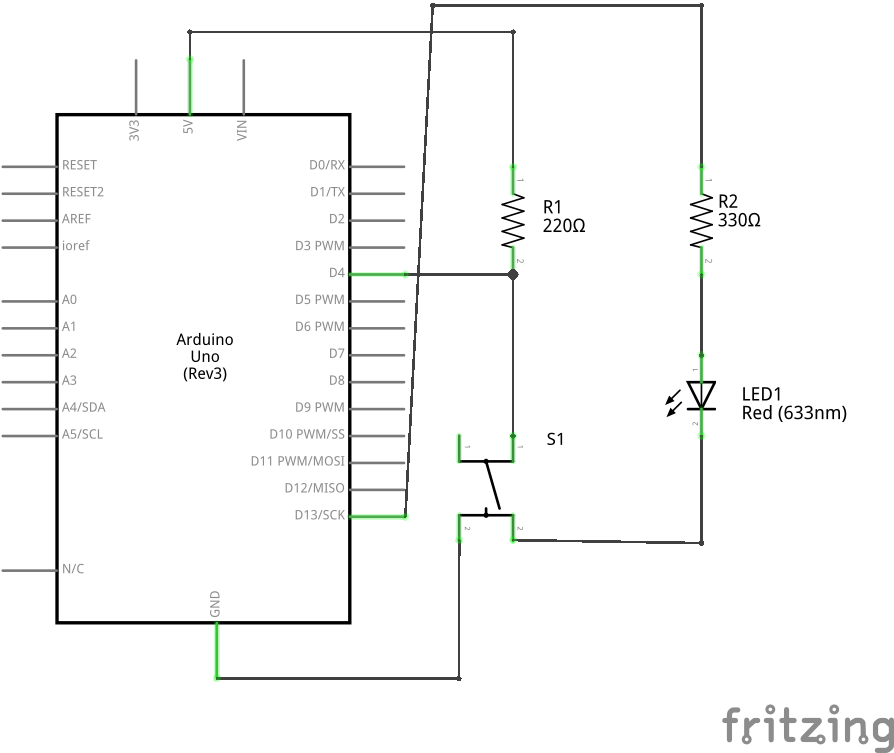
\includegraphics[width=7.0cm]{images/kadai2-2-1_kairo.png}
\caption{課題2.2.1の回路図}
\label{fig:2-2-1kairo}
\end{center}
\end{figure}


\begin{figure}[H]
\begin{center}
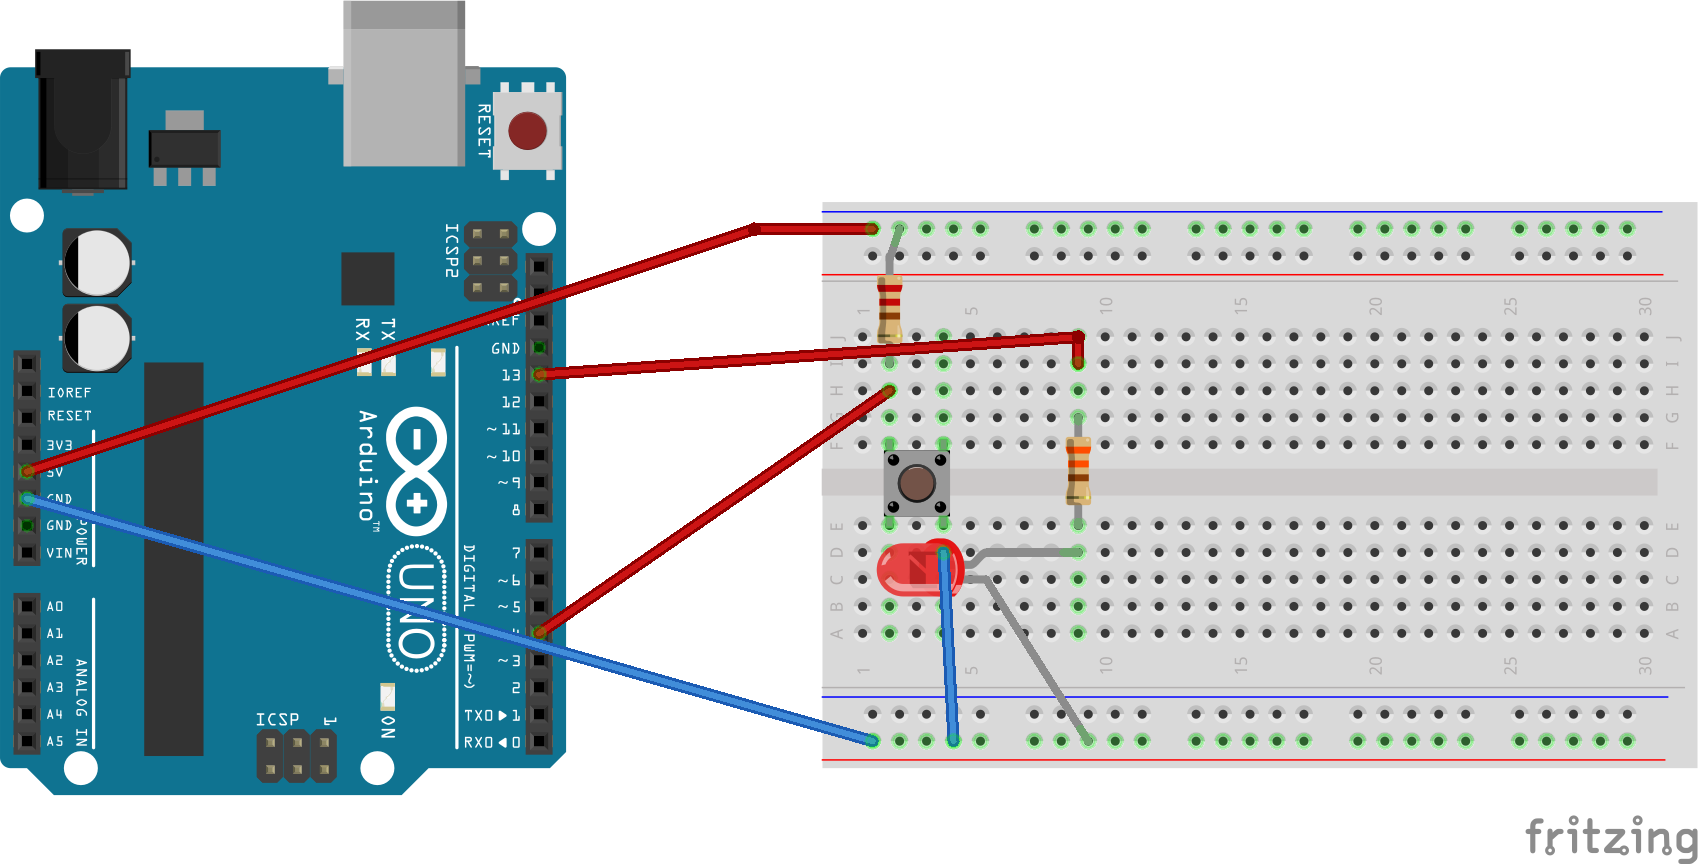
\includegraphics[width=7.0cm]{images/kadai2-2-1_bread.png}
\caption{課題2.2.1の配線図}
\label{fig:2-2-1bread}
\end{center}
\end{figure}

このLEDの動作は,13番ポートを出力として,13番ポートにHIGHを出力した後,1000ms待ち13番ポートにLOWを出力し再び1000ms待つという動作をする.

\subsection{Arduinoによるブレッドボード上のLEDの点滅}
課題2.2.2において実装した回路図,ブレッドボード配線図およびスケッチを報告せよ.また,pinMode関数の役割について考察せよ.
課題2.2.2で作成したソースコードはソースコード\ref{code:kadai2-2-2}に,回路図を\ref{fig:2-2-2kairo}に,ブレッドボード配線図を\ref{fig:2-2-2bread}にそれぞれ示す.

\begin{lstlisting}[caption = 課題2.2.2,label=code:kadai2-2-2][H]
void setup() {
  pinMode(3, OUTPUT);//13番ポートを出力に設定
}

void loop() {
  digitalWrite(3, HIGH);   // HIGHを出力
  delay(1000);                       // 1000ms待つ
  digitalWrite(3, LOW);    //LOWを出力
  delay(1000);                      //1000ms待つ
}
\end{lstlisting}

\begin{figure}[H]
\begin{center}
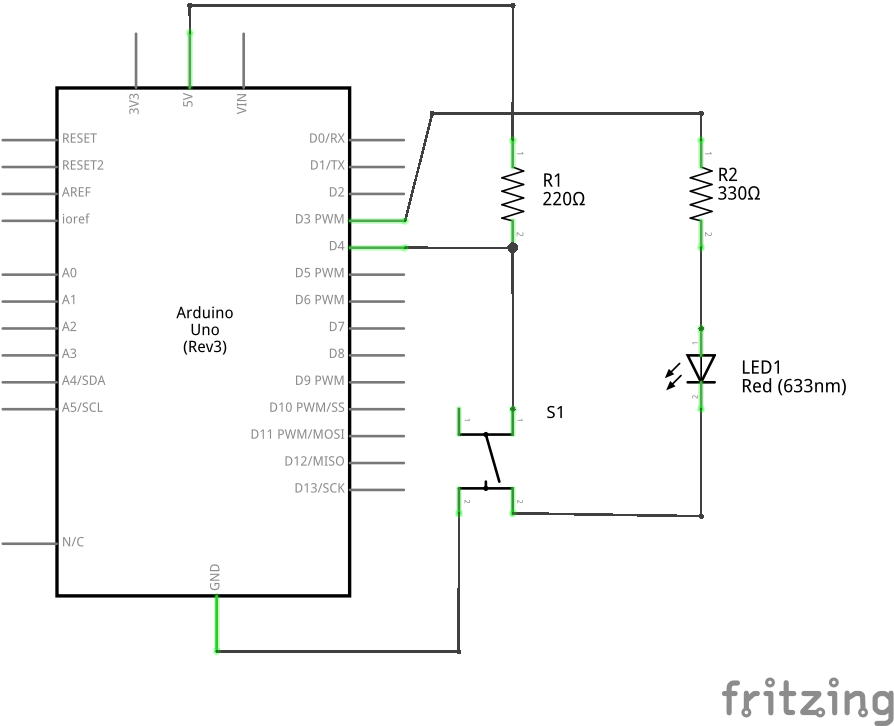
\includegraphics[width=7.0cm]{images/kadai2-2-2_kairo.png}
\caption{課題2.2.2の回路図}
\label{fig:2-2-2kairo}
\end{center}
\end{figure}

\begin{figure}[H]
\begin{center}
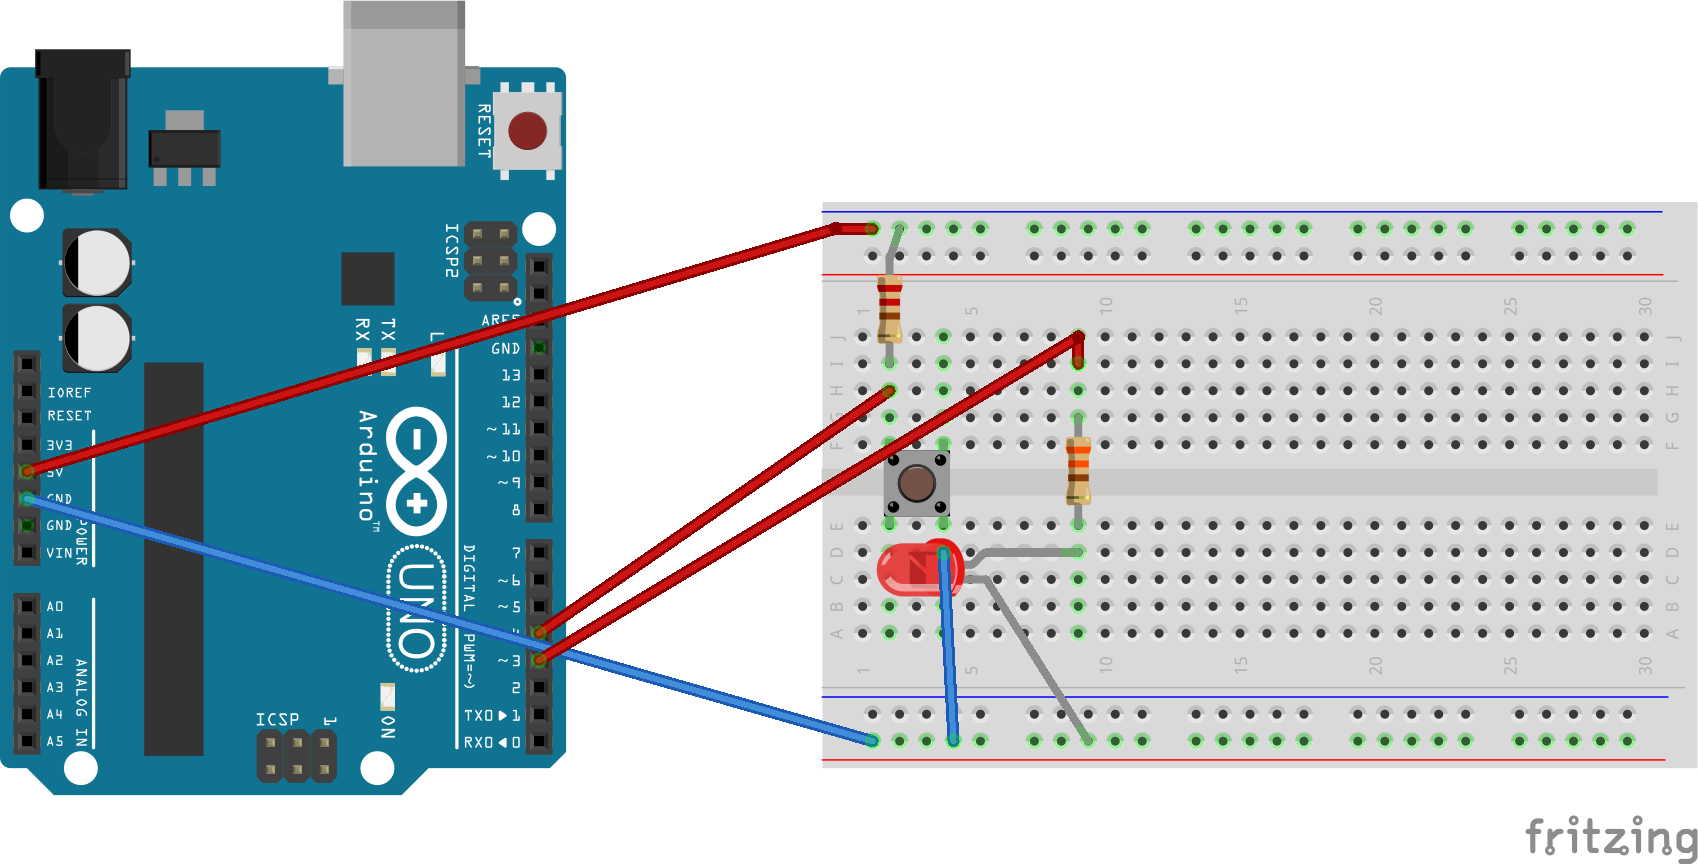
\includegraphics[width=7.0cm]{images/kadai2-2-2_bread.png}
\caption{課題2.2.2の配線図}
\label{fig:2-2-2bread}
\end{center}
\end{figure}

pinMode関数は出力や入力のポートを設定する役割があると考えられる.

\subsection{スイッチの状態をLEDに表示}
演習2.2.3で作成したスケッチを報告せよ.また,digitalRead関数の役割について考察せよ.さらにArduinoマイコンとスイッチを接続した場合のスイッチの動作原理およびマイコンへの入力信号について,回路図とスケッチより説明せよ.
演習2.2.3で作成したソースコードはソースコード\ref{code:enshu2-2-3}に示す.

\begin{lstlisting}[caption = 演習2.2.3,label=code:enshu2-2-3][H]
const int LED_PIN = 13; //LED_PINを13に定義
const int SW_PIN = 4; //SW_PINを4に定義
int sw1;//スイッチ保存用
void setup() {
  pinMode(LED_PIN,OUTPUT);//13番ポートを出力に設定
  pinMode(SW_PIN,INPUT);//4番ポートを入力に設定
}
void loop() {
  sw1=digitalRead(SW_PIN);//sw1に入力を代入
  if(sw1==LOW){
    digitalWrite(LED_PIN,HIGH);
  }
  else{
    digitalWrite(LED_PIN,LOW);
  }
}
\end{lstlisting}

digitalRead関数は引数で与えられたポートの状態を確認する役割があると考えられる,Arduinoマイコンとスイッチを接続した場合,回路はプルアップ抵抗であるためスイッチを押していないときに回路の出力はHIGHになり,スイッチが押された時回路の出力はLOWとなる.

\subsection{スイッチによるLED点灯・消灯するLEDを変更}
課題2.2.4で実装した回路図,ブレッドボード配線図およびスケッチを報告せよ.また,作成したスケッチで工夫した点を記せ.

以下に課題2.2.4で作成したソースコードをソースコード\ref{code:kadai2-2-4},回路図を図\ref{fig:kadai2-2-4kairo},配線図を図\ref{fig:kadai2-2-4bread}に示す.

\begin{lstlisting}[caption = 課題2.2.4,label=code:kadai2-2-4][H]
const int LED_RED_PIN = 3;//LED_RED_PINを3に定義
const int LED_YEL_PIN = 13;//LED_YEL_PINを13に定義
const int SW_PIN = 4; //SW_PINを4に定義
int sw1;//スイッチの入力保存用
void setup() {
  pinMode(LED_RED_PIN,OUTPUT);//LED_RED_PINを出力に設定
  pinMode(LED_YEL_PIN,OUTPUT);//LED_YEL_PINを出力に設定
  pinMode(SW_PIN,INPUT);//SW_PINを入力に設定
}
void loop() {
  sw1=digitalRead(SW_PIN);//sw1にSW_PINの値を保存
  if(sw1==LOW){//スイッチがONなら
    digitalWrite(LED_RED_PIN,HIGH);//赤をHIGH
    digitalWrite(LED_YEL_PIN,LOW);//黄色をLOW
  }
  else{
    digitalWrite(LED_RED_PIN,LOW);//赤をLOW
    digitalWrite(LED_YEL_PIN,HIGH);//黄色HIGH
  }
}
\end{lstlisting}

\begin{figure}[H]
\begin{center}
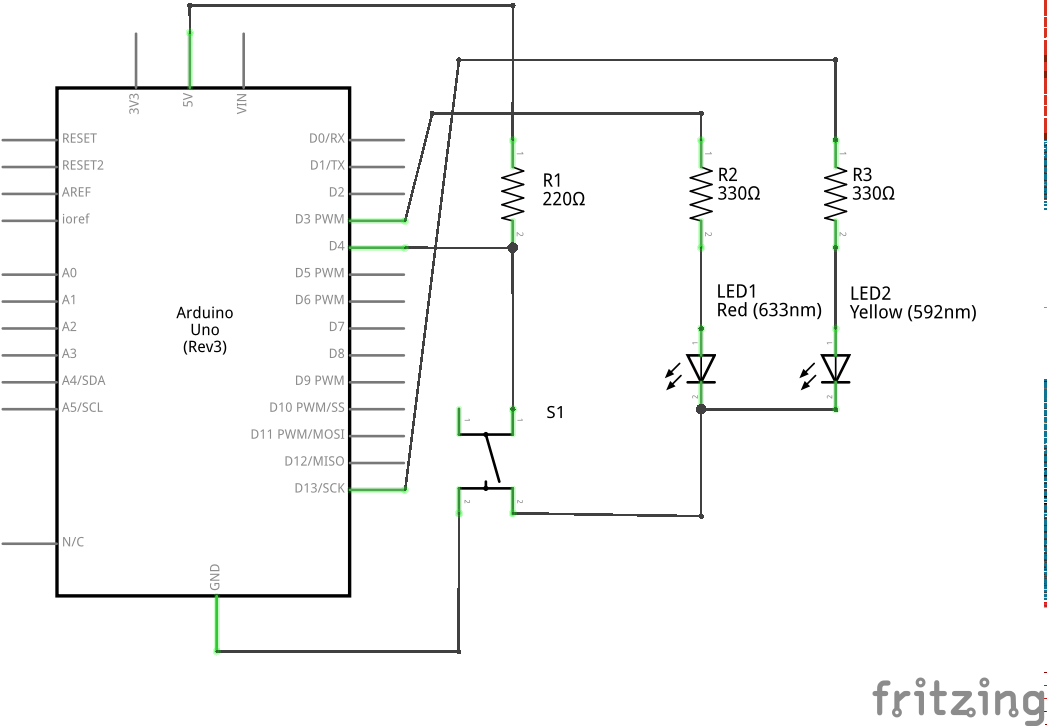
\includegraphics[width=7.0cm]{images/kadai2-2-4_kairo.png}
\caption{課題2.2.4の回路図}
\label{fig:kadai2-2-4kairo}
\end{center}
\end{figure}

\begin{figure}[H]
\begin{center}
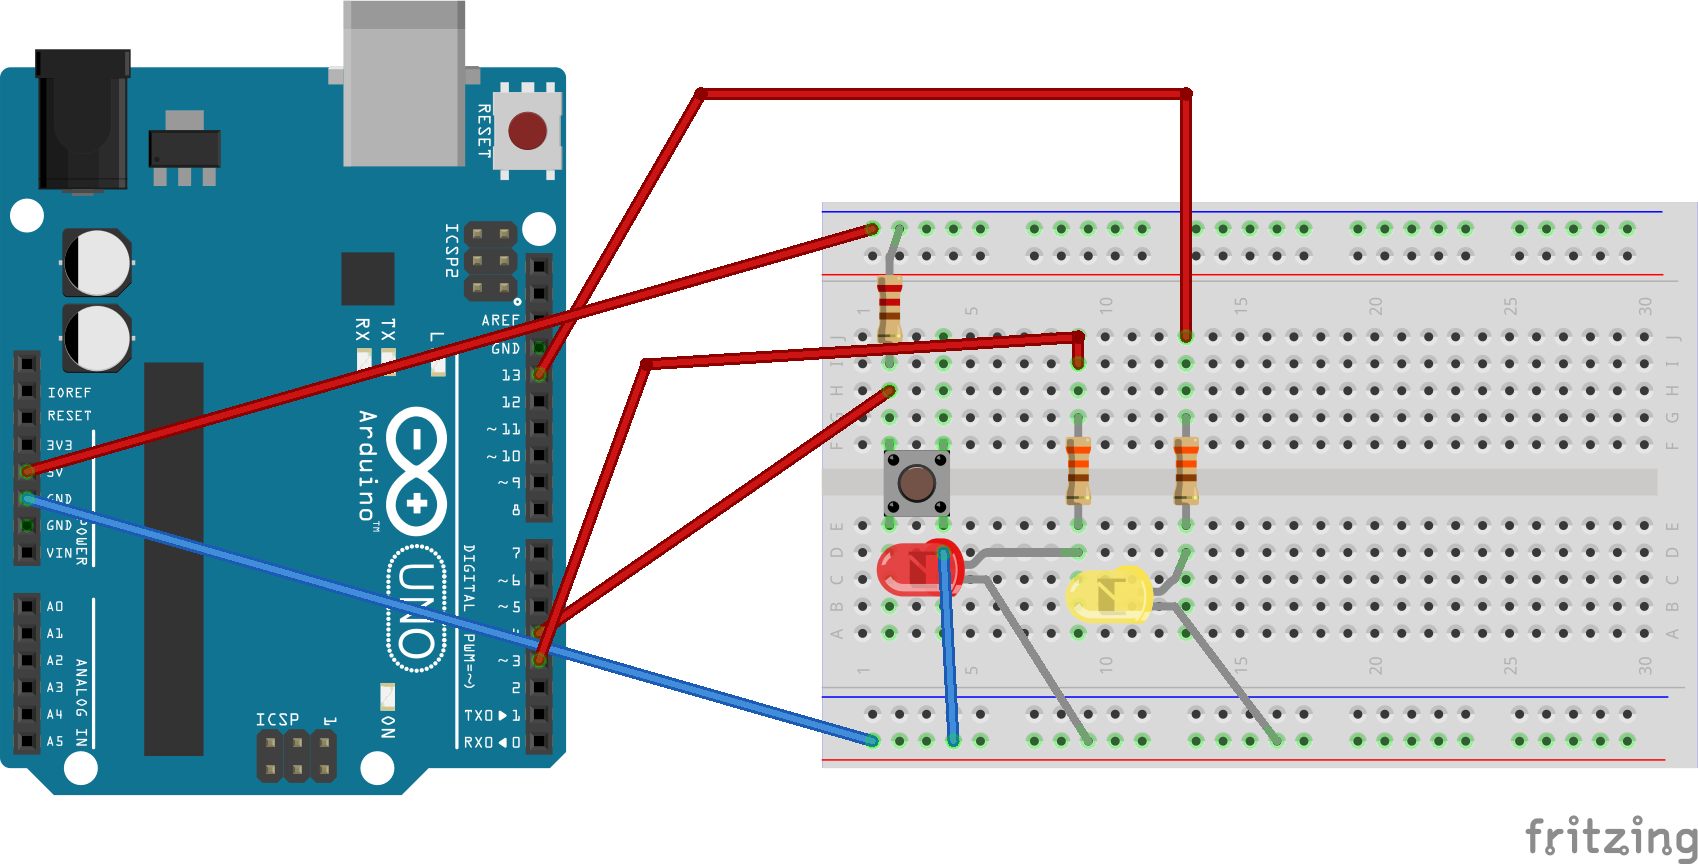
\includegraphics[width=7.0cm]{images/kadai2-2-4_bread.png}
\caption{課題2.2.4の配線図}
\label{fig:kadai2-2-4bread}
\end{center}
\end{figure}

\subsection{forループを用いて点数回数を制御}
発展課題2.2.1のスケッチを報告せよ.またスケッチで工夫した点を記せ.

以下ソースコード\ref{code:hatten2-2-1}にソースコードを示す.

\begin{lstlisting}[caption = 発展2.2.1,label=code:hatten2-2-1][H]
const int LED_PIN = 3;
void setup() {
  pinMode(LED_PIN,OUTPUT);
}

void loop() {
  for(int i = 0; i <= 5;i++){
    digitalWrite(LED_PIN,HIGH);
    delay(500);
    digitalWrite(LED_PIN,LOW);
    delay(500);
  }
  delay(2000);
}
\end{lstlisting}

特に工夫したというわけではないが,簡潔で誰でも分かりやすいようなプログラムにした.

\subsection{スイッチ2個,LED1個による論理回路}
発展課題2.2.2で実装した回路図,ブレッドボード配線図およびスケッチを報告せよ.また,各論理演算の式を記し表2.14,2.15の結果を報告せよ.さらに作成したスケッチで工夫した点を記せ.

以下ソースコード\ref{code:hatten2-2-2-1},\ref{code:hatten2-2-2-2}にそれぞれソースコードを,
図\ref{fig:hatten2-2-2kairo}に回路図を,図\ref{fig:hatten2-2-2bread}に配線図をそれぞれ示す.



\begin{lstlisting}[caption = 発展課題2(AND),label=code:hatten2-2-2-1][H]
const int SW1_PIN = 3; 
const int SW2_PIN = 4;
const int LED_PIN = 13;
int sw1;
int sw2;//使うものを定義
void setup() {
  pinMode(SW1_PIN,INPUT);
  pinMode(SW2_PIN,INPUT);
  pinMode(LED_PIN,OUTPUT);//入出力関係
}

void loop() {
  sw1=digitalRead(SW1_PIN);
  sw2=digitalRead(SW2_PIN);//読み込み
  if(sw1==LOW&&sw2==LOW){//1,1
    digitalWrite(LED_PIN,HIGH);
  }
  if(sw1==LOW&&sw2==HIGH){//1,0
    digitalWrite(LED_PIN,HIGH);
  }
  if(sw1==HIGH&&sw2==LOW){//0,1
    digitalWrite(LED_PIN,HIGH);
  }
  if(sw1==HIGH&&sw2==HIGH){//0,0
    digitalWrite(LED_PIN,LOW);
  }
}
\end{lstlisting}

\begin{lstlisting}[caption = 発展課題2(OR),label=code:hatten2-2-2-2][H]
const int SW1_PIN = 3;
const int SW2_PIN = 4;
const int LED_PIN = 13;
int sw1;
int sw2;//使うものを定義
void setup() {
  pinMode(SW1_PIN,INPUT);
  pinMode(SW2_PIN,INPUT);
  pinMode(LED_PIN,OUTPUT);//入出力関係
}

void loop() {
  sw1=digitalRead(SW1_PIN);
  sw2=digitalRead(SW2_PIN);
  if(sw1==LOW&&sw2==LOW){//1,1
    digitalWrite(LED_PIN,HIGH);
  }
  if(sw1==LOW&&sw2==HIGH){//1,0
    digitalWrite(LED_PIN,LOW);
  }
  if(sw1==HIGH&&sw2==LOW){//0,1
    digitalWrite(LED_PIN,LOW);
  }
  if(sw1==HIGH&&sw2==HIGH){//0,0
    digitalWrite(LED_PIN,LOW);
  }
}
\end{lstlisting}

\begin{figure}[H]
\begin{center}
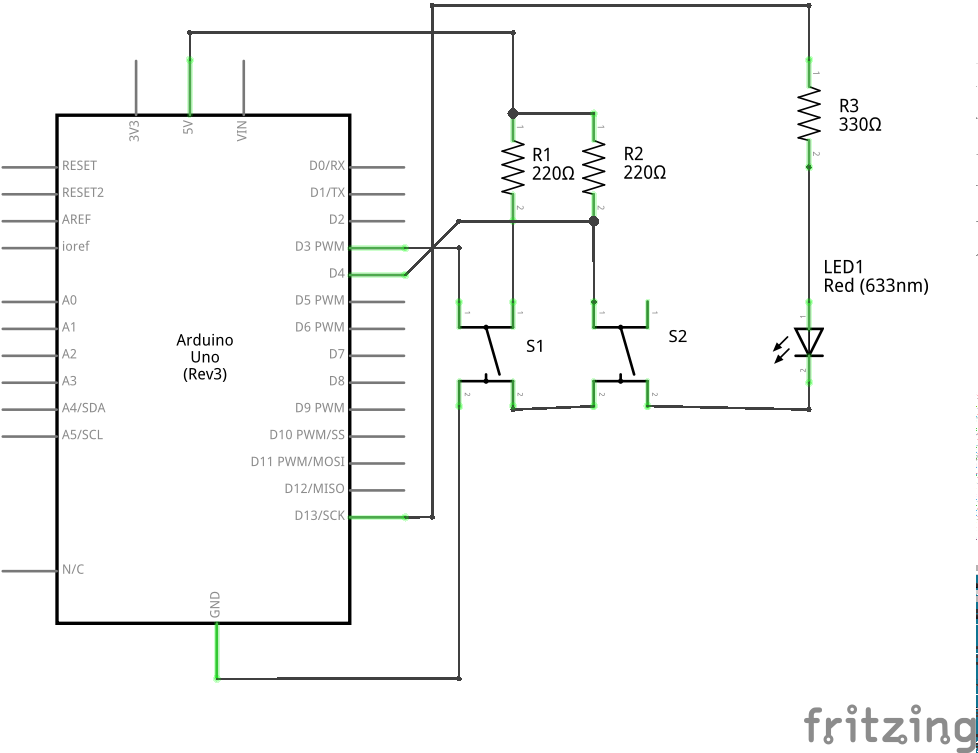
\includegraphics[width=7.0cm]{images/hatten2-2-2_kairo.png}
\caption{発展2.2.2の回路図}
\label{fig:hatten2-2-2kairo}
\end{center}
\end{figure}

\begin{figure}[H]
\begin{center}
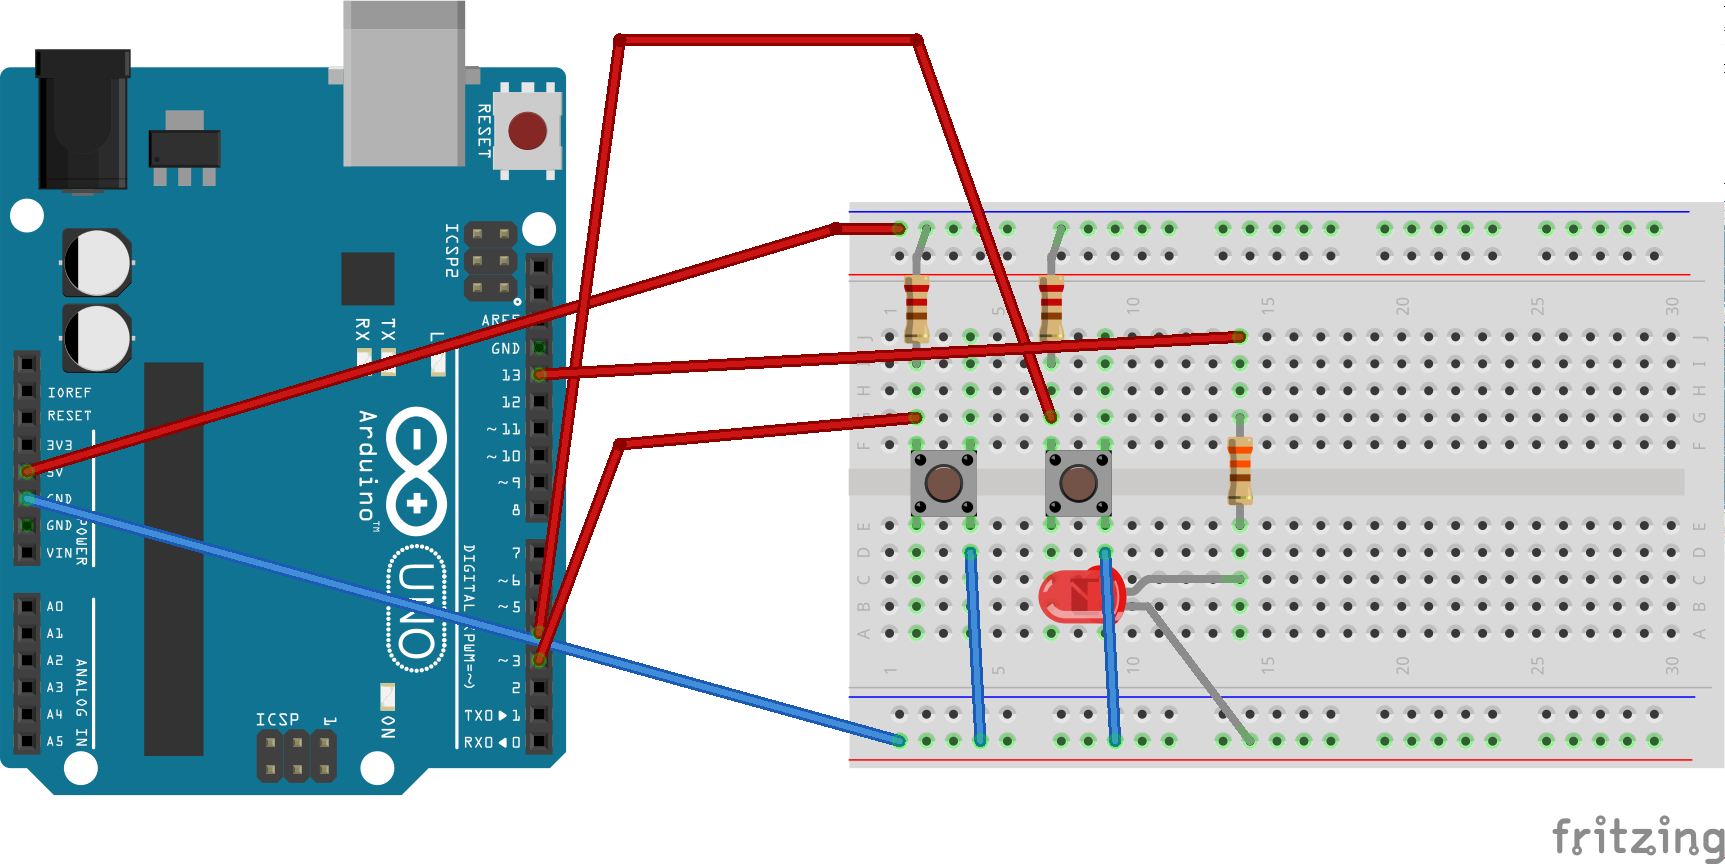
\includegraphics[width=7.0cm]{images/hatten2-2-2_bread.png}
\caption{発展2.2.2の配線図}
\label{fig:hatten2-2-2bread}
\end{center}
\end{figure}

また結果を表\ref{table:and},表\ref{table:or}にそれぞれ示す.

\begin{table}[H]
\centering
\caption{AND}
\label{table:and}
\begin{center}
\begin{tabular}{c|c|c}
\hline \hline
SW1 & SW2 & LED1\\ \hline
ON & ON &点灯 \\
ON& OFF & 消灯 \\
OFF& ON& 消灯\\
OFF& OFF & 消灯\\ \hline
\end{tabular}
\end{center}
\end{table}

\begin{table}[H]
\centering
\caption{OR}
\label{table:or}
\begin{center}
\begin{tabular}{c|c|c}
\hline \hline
SW1 & SW2 & LED1\\ \hline
ON & ON &点灯 \\
ON& OFF & 点灯 \\
OFF& ON& 点灯\\
OFF& OFF & 消灯\\ \hline
\end{tabular}
\end{center}
\end{table}
分かりやすいように工夫はしたが,その分if文を4つ使ってしまい冗長なプログラムとなってしまった.
\subsection{回路実装およびプログラム作成状態の報告}
うまく実装および作成できたか?どの部分の実装,プログラム作成が失敗または難しかったか?

今回は比較的簡単な回路と簡単なプログラムだったため特につまずくことはなかったが,何か問題が生じた時それがソフトの問題なのかハードの問題なのかしっかりと見極める必要があるなと感じた.

\end{document}
